% !TEX root = ../thesis-example.tex
%
\chapter{Introduction}\label{sec:intro}
During the past decade, the use of artificial intelligence (AI) and machine learning (ML) methods has spread across various sectors, driving innovation and efficiency at unprecedented scales.
The development of hardware components such as Graphical Processing Units (GPUs) and Tensor Processing Units (TPUs), combined with the availability of large amounts of data has shown the potential of Machine Learning models to uncover latent patterns in data, and has 
driven advancements in fields such as image and natural language processing, autonomous driving, healthcare, and finance. A particular class of ML models, termed as generative modeling, has shown promise in the recent years by its ability to generate realistic samples by training on a dataset.
\\
Generative modeling is a subfield of machine learning that focuses on learning the underlying distribution of a dataset to generate new samples. It has proven to be effective for numerous types of data, including language \citep{openai2024gpt4technicalreport}, image generation \citep{rombach2022highresolutionimagesynthesislatent}, and drug discovery \citep{jumper2021highly}.
Recent generative models are based on neural networks, and prominent models include Generative Adversarial Networks (GANs) \citep{goodfellow2014generativeadversarialnetworks}, Variational Auto-Encoder (VAEs) \citep{Kingma_2019}, and Diffusion models \citep{song2021scorebasedgenerativemodelingstochastic}.
\\
The success of generative models hides their training procedure that is usually long, computationally expensive, and requires a large amount of data. The training of generative models is challenging due to the high-dimensional nature of the data and the need to learn complex distributions. For instance, figure \ref{fig:expo_parameters} displays an exponential increase on the number of parameters of architectures involved in generative models.
This raises numerous questions on the \textit{frugality} of the training procedure. Several research directions have been proposed to address this issue, including the use of transfer learning \citep{zhuang2020comprehensivesurveytransferlearning}, neural architecture search \citep{verbockhaven2024growingtinynetworksspotting} and pruning methods \citep{sun2024simpleeffectivepruningapproach}.
\begin{figure}[t]
    \centering
    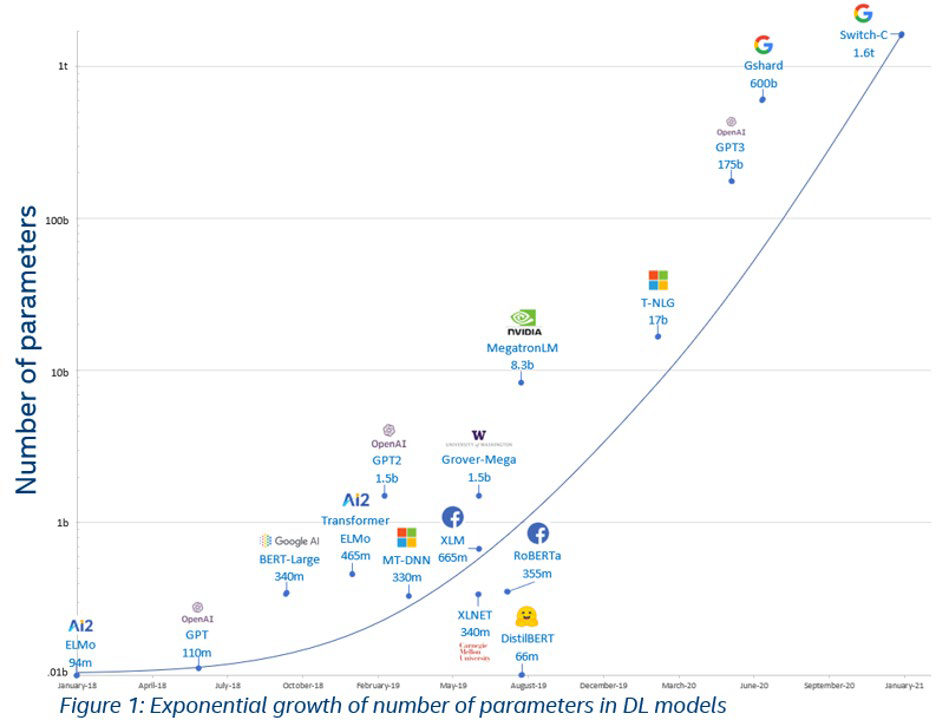
\includegraphics[width=\textwidth]{gfx/expo_parameters.png}
    \caption{Number of parameters of architectures used in large language models. Source: \url{https://www.webagesolutions.com/blog/generative-ai-engineering}}
    \label{fig:expo_parameters}
\end{figure}
\\

In this work, we focus on a subset of generative models, that is diffusion models. Diffusion models consists in 
gradually adding noise to the data and then learning to reverse this process to reconstruct the original data. This type of model has gained attention for its potential to generate high-quality and diverse samples, while providing a theoretically sound framework based on Markov chains \citep{ho2020denoisingdiffusionprobabilisticmodels} and stochastic differential equations \citep{song2021scorebasedgenerativemodelingstochastic}. 
We are particularly interested in developing methods to refine a pre-trained diffusion model without re-training it. That is, improve its generation abilities without using the important computational power required to train the whole model.
More specifically, we aim to investigate the potential of using boosting methods, i.e using auxiliary smaller models, to improve the generation capabilities of a pre-trained diffusion model. A smaller model will thus act as correcting the errors made by the pre-trained model. 
\\
The main sources of error that a diffusion model can make stem from \textit{approximation} erros and \textit{sampling} errors. Approximation errors denote the accuracy of estimation of the score compnent during the training phase, and sampling errors refer to the errors made during the sampling phase. 
We thus raise the following question : 
\begin{center}
    \textbf{Can we devise boosting methods to correct the errors made by a pre-trained diffusion model ?}
\end{center}
We answer to this question by presenting two methods : discriminator guidance and f-Restart sampling. The former method attemps to correct the approximation error by using a smaller discriminator network to correct the score. f-Restart sampling attempts to correct the sampling error by using a reinforcement learning procedure during the sampling process, deciding between performing a denoising step or injecting noise as a correction term.
The structure of our thesis is as follows : \begin{itemize}
    \item \textbf{Chapter \ref{sec:diffusion} :} In this section, we give an overview of generative models, then present the derivation of diffusion models. Then, we list a few refinement methods proposed for generative models that are based on density ratio estimation technique, motivating the use of a discriminator.
    \item \textbf{Chapter \ref{sec:dg} :} In this section, we present discriminator guidance as a method for correcting the approximation error involved in training a score network. We improve upon previous results by deriving an optimal objective function, and we expose the experimental results on standard image generation benchmarks.
    \item \textbf{Chapter \ref{sec:rl} :} In this section, we present restart sampling as a boosting-free method for refining the sampling error of a diffusion model. We then propose $f-$Restart sampling, a method that improves upon the previous one by incorporating a reinforcement learning algorithm to dynamically denoise samples.
\end{itemize}
